\documentclass[conference]{IEEEtran}

% ============================================================
% PAQUETES
% ============================================================
\usepackage[utf8]{inputenc}
\usepackage[T1]{fontenc}
\usepackage[spanish]{babel}
\usepackage{graphicx}
\usepackage{amsmath}
\usepackage{amssymb}
\usepackage{booktabs}
\usepackage{array}

% Decimales con punto, en coherencia con las figuras y con el estilo IEEE
\spanishdecimal{.}

% Rotulación de figuras y tablas al estilo IEEE (babel la redefine al inicio)
\addto\captionsspanish{%
  \renewcommand{\figurename}{Fig.}%
  \renewcommand{\tablename}{Tabla}%
}
\renewcommand{\IEEEkeywordsname}{Palabras clave}

% Ruta de las figuras
\graphicspath{{../figs/}}

\begin{document}

% ============================================================
% TÍTULO Y AUTOR
% ============================================================
\title{Corrección de errores cuánticos y tasa de clave segura en BB84 bajo canales ruidosos}

\author{
\IEEEauthorblockN{Eliu Manuel Pat Ojeda}
\IEEEauthorblockA{\textit{Maestría en Ciberseguridad}\\
\textit{Universidad Tecnológica Metropolitana}\\
Mérida, Yucatán, México}
}

\maketitle

% ============================================================
% RESUMEN
% ============================================================
\begin{abstract}
El advenimiento del cómputo cuántico, sintetizado en la noción de \textit{Q-Day},
compromete los esquemas de clave pública que sostienen la infraestructura
digital. La distribución de claves cuánticas (QKD) ofrece una alternativa cuya
seguridad no depende de supuestos computacionales, pero su viabilidad práctica
está limitada por el ruido del canal, que eleva la tasa de error de bit cuántico
(QBER) y reduce la clave secreta disponible. La corrección de errores cuánticos
(QEC) mitiga ese efecto a costa de un \textit{overhead} de qubits que penaliza la
tasa efectiva. Este trabajo cuantifica ese compromiso para el protocolo BB84
sobre un canal depolarizante, mediante simulación con QuTiP de códigos de
repetición con $n = 3, 5$ y $7$. Los resultados muestran que no existe un tamaño
de código universalmente óptimo: para $p \leq 0.10$ conviene operar sin
corrección, entre $0.12$ y $0.18$ el óptimo es $n = 3$, entre $0.20$ y $0.26$ lo
es $n = 5$, y desde $0.28$ domina $n = 7$. La corrección, además, desplaza el
umbral de seguridad más allá de $p = 0.30$, lo que aproximadamente duplica la
tolerancia al ruido del enlace.
\end{abstract}

\begin{IEEEkeywords}
Distribución de claves cuánticas, protocolo BB84, corrección de errores
cuánticos, Q-Day, tasa de clave segura.
\end{IEEEkeywords}

% ============================================================
% INTRODUCCIÓN
% ============================================================
\section{Introducción}

La seguridad de la infraestructura digital contemporánea descansa sobre un
conjunto reducido de supuestos matemáticos. Los esquemas de clave pública que
sostienen las comunicaciones cifradas, la firma electrónica y los sistemas de
control industrial fundan su fortaleza en la dificultad computacional de
factorizar enteros grandes y de resolver el logaritmo discreto. \cite{shor1997}
demostró que ambos problemas admiten solución en tiempo polinómico sobre un
computador cuántico suficientemente grande y tolerante a fallos. El horizonte en
que dicha capacidad esté disponible se designa como \textit{Q-Day}: a partir de
él, los algoritmos mencionados dejan de ofrecer garantías de confidencialidad
para los datos que protegen.

La amenaza no pertenece únicamente al futuro. La estrategia \textit{Harvest Now,
Decrypt Later} consiste en interceptar y archivar tráfico cifrado en el presente
para descifrarlo cuando se disponga de capacidad cuántica \cite{mosca2018}. El
criterio decisivo no es la fecha del Q-Day, sino la relación entre el tiempo
requerido para migrar la infraestructura y el periodo durante el cual los datos
deben permanecer secretos; cuando el segundo excede al primero, la información ya
se encuentra comprometida aunque su contenido aún no pueda leerse. Por esa razón,
el informe NIST IR 8547 recomienda iniciar la transición criptográfica antes de
que exista una amenaza operativa confirmada \cite{regenscheid2026}.

La respuesta institucional se ha articulado en torno a la criptografía
post-cuántica, con la publicación de los estándares FIPS 203 y FIPS 204
\cite{nist2024a,nist2024b}. Se trata, sin embargo, de una solución algorítmica:
su seguridad vuelve a descansar en supuestos de complejidad computacional que,
aunque más robustos, no son indemnes a futuros avances del cómputo cuántico.
Frente a ese enfoque, la distribución de claves cuánticas (QKD) propone un
fundamento distinto: la seguridad se deriva de las leyes de la mecánica cuántica
y no de la dificultad de un problema matemático. El protocolo BB84
\cite{bennett1984} permite a dos partes acordar una clave mediante estados
cuánticos codificados en dos bases no ortogonales; el teorema de no-clonación y
la perturbación inevitable de la medición garantizan que cualquier intento de
interceptación introduzca errores detectables \cite{gisin2002}. Su seguridad
incondicional fue demostrada por \cite{shor2000}, y las condiciones de seguridad
práctica han sido precisadas en revisiones posteriores \cite{scarani2009,xu2020}.

La viabilidad de la QKD depende de la calidad del canal. En fibra óptica, la
atenuación, la decoherencia, el desalineamiento de los componentes ópticos y las
cuentas oscuras de los detectores introducen discrepancias entre los bits
preparados por Alice y los medidos por Bob \cite{xu2020}. Esas discrepancias se
cuantifican mediante la tasa de error de bit cuántico (QBER), y su magnitud
condiciona la fracción de bits que puede convertirse en clave secreta: superado
un umbral cercano al 11\,\%, la tasa de clave segura se anula \cite{shor2000}.
La corrección de errores cuánticos (QEC) es el mecanismo que permite operar por
debajo de ese umbral \cite{nielsen2010,terhal2015}, y su madurez tecnológica
quedó demostrada con la supresión del error lógico bajo el umbral del código de
superficie en un procesador superconductor \cite{acharya2025}.

La corrección tiene un costo. Un código de repetición de $n$ qubits emplea $n$
qubits físicos por qubit lógico, de modo que la tasa efectiva queda penalizada
por un factor $1/n$ \cite{fowler2012}. Incrementar $n$ reduce el QBER residual
pero también reduce el número de bits de clave por qubit transmitido, de manera
que la tasa efectiva no es monótona en $n$. Los trabajos recientes han abordado
componentes aislados de este problema, pero ninguno establece la frontera que
relaciona el ruido del canal con el tamaño de código que maximiza la tasa
efectiva, como se detalla en la Sección~\ref{sec:antecedentes}.

Este trabajo cubre ese vacío. Su contribución es cuantificar, mediante
simulación, la frontera de optimalidad $n^{*}(p)$ del código de repetición en
BB84 sobre un canal depolarizante, y derivar de ella criterios de
dimensionamiento para sistemas de QKD. El resto del artículo se organiza como
sigue: la Sección~\ref{sec:antecedentes} revisa los antecedentes; la
Sección~\ref{sec:metodo} describe el modelo y la estrategia metodológica; la
Sección~\ref{sec:resultados} presenta los resultados; y la
Sección~\ref{sec:conclusion} expone las conclusiones.

% ============================================================
% ANTECEDENTES
% ============================================================
\section{Antecedentes}
\label{sec:antecedentes}

La intersección entre corrección de errores y distribución de claves cuánticas
es un área de investigación reciente, y los trabajos disponibles abordan
componentes aislados del problema. \cite{jha2024} propusieron integrar el cifrado
y la corrección en un mismo proceso mediante códigos CSS, con el objetivo de
reducir el costo total al evitar etapas separadas. Su enfoque ataca el costo
fijo de la arquitectura, pero no analiza cómo varía el tamaño de bloque óptimo
con el ruido del canal.

\cite{zheng2024} desarrollaron una métrica de fidelidad de canal casi óptima que
permite evaluar el desempeño de un código sin resolver problemas de optimización
costosos. Se trata de una herramienta valiosa para comparar códigos, aunque su
métrica es la fidelidad y no la tasa de clave; en consecuencia, no incorpora el
costo en qubits que resulta determinante en un enlace de QKD.

\cite{jayachandran2025} validaron experimentalmente la aplicación de QEC en BB84
y reportaron la reducción del QBER con el consiguiente incremento de la tasa de
clave. Su aportación confirma la dirección del presente trabajo, pero no
construye la frontera de optimalidad en función de $p$ ni cuantifica el efecto
sistemático del \textit{overhead}.

Finalmente, \cite{acharya2025} demostraron la supresión del error lógico bajo el
umbral del código de superficie en un procesador superconductor de 105 qubits.
El resultado valida la viabilidad de la QEC en hardware, aunque en un régimen
distinto al de un enlace de comunicación: allí se persigue la fidelidad de un
computador tolerante a fallos, con decenas o centenas de qubits físicos por qubit
lógico, mientras que en QKD basta con proteger el bit transmitido.

En conjunto, la literatura acredita que la QEC mejora la fiabilidad y que puede
incrementar la tasa de clave, pero no establece, para BB84, la relación entre el
nivel de ruido y el tamaño de código que maximiza la tasa efectiva. Esa frontera
es la que este trabajo determina.

% ============================================================
% MÉTODO
% ============================================================
\section{Método}
\label{sec:metodo}

\subsection{Modelo del protocolo BB84}

Alice codifica cada bit en uno de cuatro estados, eligiendo al azar una de dos
bases mutuamente no ortogonales: $Z$, formada por $\{|0\rangle,|1\rangle\}$, y
$X$, formada por $\{|+\rangle,|-\rangle\}$, con
$|\pm\rangle=(|0\rangle\pm|1\rangle)/\sqrt{2}$. Bob mide en una base elegida de
forma independiente y, tras el cribado (\textit{sifting}), ambas partes
conservan solo los bits en los que coincidieron. Sobre esa muestra se estima el
QBER y se aplica el post-procesamiento.

La seguridad se reduce a la de un código de corrección de errores
\cite{shor2000}. En el límite asintótico, la fracción de bits aprovechables como
clave secreta satisface
\begin{equation}
R = 1 - 2H_2(\mathrm{QBER}),
\label{eq:shor}
\end{equation}
donde $H_2(x) = -x\log_2 x - (1-x)\log_2(1-x)$ es la entropía binaria de
Shannon. De \eqref{eq:shor} se sigue que la tasa es positiva solo si
$\mathrm{QBER} < 11$\,\% aproximadamente.

\subsection{Canal depolarizante}

El ruido se modela con un canal depolarizante, que actúa sobre un qubit según
\begin{equation}
\mathcal{E}(\rho) = (1-p)\rho + \frac{p}{3}\left(X\rho X + Y\rho Y + Z\rho Z
\right),
\label{eq:canal}
\end{equation}
donde $p$ es la probabilidad de que ocurra un error de Pauli y cada operador se
aplica con probabilidad $p/3$ \cite{nielsen2010}. En BB84, un error de bit se
produce si el qubit sufre $X$ o $Y$, mientras que un error $Z$ altera únicamente
la fase; en consecuencia, la discrepancia entre Alice y Bob es
\begin{equation}
\mathrm{QBER} = \frac{2}{3}p .
\label{eq:qber}
\end{equation}

\subsection{Código de repetición}

El código empleado es el de repetición de $n$ qubits, que codifica
\begin{equation}
|0\rangle_L = |00\cdots 0\rangle, \qquad
|1\rangle_L = |11\cdots 1\rangle,
\label{eq:codigo}
\end{equation}
y cuyo estabilizador está generado por $g_i = Z_iZ_{i+1}$, con
$i=1,\ldots,n-1$. La medición de esos generadores produce un síndrome de $n-1$
bits que identifica el qubit afectado, tras lo cual se aplica la corrección y se
decodifica por votación mayoritaria \cite{nielsen2010}. El código corrige hasta
$t=\lfloor (n-1)/2 \rfloor$ errores de bit y, bajo el supuesto de errores
independientes con probabilidad $q$ por qubit físico, su probabilidad de fallo
lógico es
\begin{equation}
P_{\text{fallo}}(n,q) = \sum_{k=\lceil n/2 \rceil}^{n} \binom{n}{k}
q^{k}(1-q)^{n-k}.
\label{eq:fallo}
\end{equation}

\subsection{Tasa de clave efectiva}

El \textit{overhead} se introduce como el factor de eficiencia
$\eta(n)=1/n$, que penaliza la tasa de clave. Combinándolo con \eqref{eq:shor} se
obtiene la métrica central del estudio:
\begin{equation}
R_{\text{efectiva}}(p,n)
= \frac{1}{n}\left[1 - 2H_2\left(\mathrm{QBER}_{\text{QEC}}(p,n)\right)\right].
\label{eq:efectiva}
\end{equation}
La inspección de \eqref{eq:efectiva} revela el compromiso: al aumentar $n$, el
QBER residual decrece y el corchete se aproxima a la unidad, pero el factor $1/n$
reduce proporcionalmente el rendimiento. Para cada $p$ debe existir, por tanto,
un tamaño de código que maximice el producto.

\subsection{Implementación y diseño experimental}

El simulador se desarrolló en Python 3.14 con la biblioteca QuTiP 5.0, que
permite representar matrices de densidad, canales cuánticos y entropías
\cite{johansson2012}. El flujo comprende cinco etapas: preparación del estado,
aplicación del canal depolarizante, medición de síndromes, corrección y
decodificación.

El diseño es experimental de simulación. Las variables independientes son la
probabilidad de error $p$, evaluada en $\{0.00, 0.02,\ldots,0.30\}$ (16 valores),
y el tamaño de código $n \in \{1,3,5,7\}$, donde $n=1$ representa la operación
sin corrección y constituye la referencia de comparación. La variable dependiente
es $R_{\text{efectiva}}$. Se transmitieron $N=10\,000$ qubits por combinación, de
los cuales aproximadamente la mitad ($\sim 5000$) sobrevivieron al cribado al
coincidir las bases; el QBER y las tasas se calcularon sobre ese subconjunto. En
total se ejecutaron 64 combinaciones de $(p,n)$.

El módulo sin corrección se validó contra \eqref{eq:qber}: el QBER simulado se
mantuvo dentro de $0.01$ del valor teórico en los 16 valores de $p$. El código de
repetición se validó con pruebas unitarias en los casos sin ruido, con error
inyectado y con ruido extremo ($p=0.9$).

% ============================================================
% RESULTADOS
% ============================================================
\section{Resultados}
\label{sec:resultados}

\subsection{Validación del simulador}

Antes de presentar el efecto de la corrección, se verificó que el módulo sin
corrección reproduce la predicción analítica de \eqref{eq:qber}. La
Tabla~\ref{tab:validacion} contrasta ambos valores en seis niveles de ruido. La
desviación absoluta se mantiene por debajo de $0.005$ en todos los casos, lo que
confirma que el generador de estados, el canal y la medición están correctamente
implementados y que las diferencias observadas en el resto del estudio son
atribuibles al efecto de la corrección y no a un sesgo del simulador.

\begin{table}[!t]
\renewcommand{\arraystretch}{1.15}
\caption{Validación del módulo sin corrección}
\label{tab:validacion}
\centering
\begin{tabular}{@{}cccc@{}}
\toprule
$p$ & QBER teórico & QBER simulado & $|\Delta|$ \\
\midrule
$0.02$ & $0.0133$ & $0.0148$ & $0.0015$ \\
$0.06$ & $0.0400$ & $0.0401$ & $0.0001$ \\
$0.10$ & $0.0667$ & $0.0704$ & $0.0038$ \\
$0.16$ & $0.1067$ & $0.1025$ & $0.0041$ \\
$0.20$ & $0.1333$ & $0.1304$ & $0.0029$ \\
$0.30$ & $0.2000$ & $0.2025$ & $0.0025$ \\
\bottomrule
\end{tabular}
\end{table}

\subsection{Reducción del QBER}

La Fig.~\ref{fig:qber} presenta el QBER medido en función de $p$ para los cuatro
escenarios. Sin corrección ($n=1$), el QBER crece de forma casi lineal con $p$,
conforme a \eqref{eq:qber}, y corta el umbral de seguridad en torno a
$p=0.16$; a partir de ese punto el enlace no puede generar clave aunque su
hardware opere correctamente. Las curvas de $n=3$, $5$ y $7$ se mantienen
notablemente planas y por debajo del umbral: en $p=0.06$ el QBER desciende de
$0.040$ a $0.003$ con $n=3$, más de diez veces menor, y en $p=0.30$ pasa de
$0.202$ a $0.092$, $0.057$ y $0.035$ para $n=3$, $5$ y $7$, respectivamente.

\begin{figure}[!t]
\centering
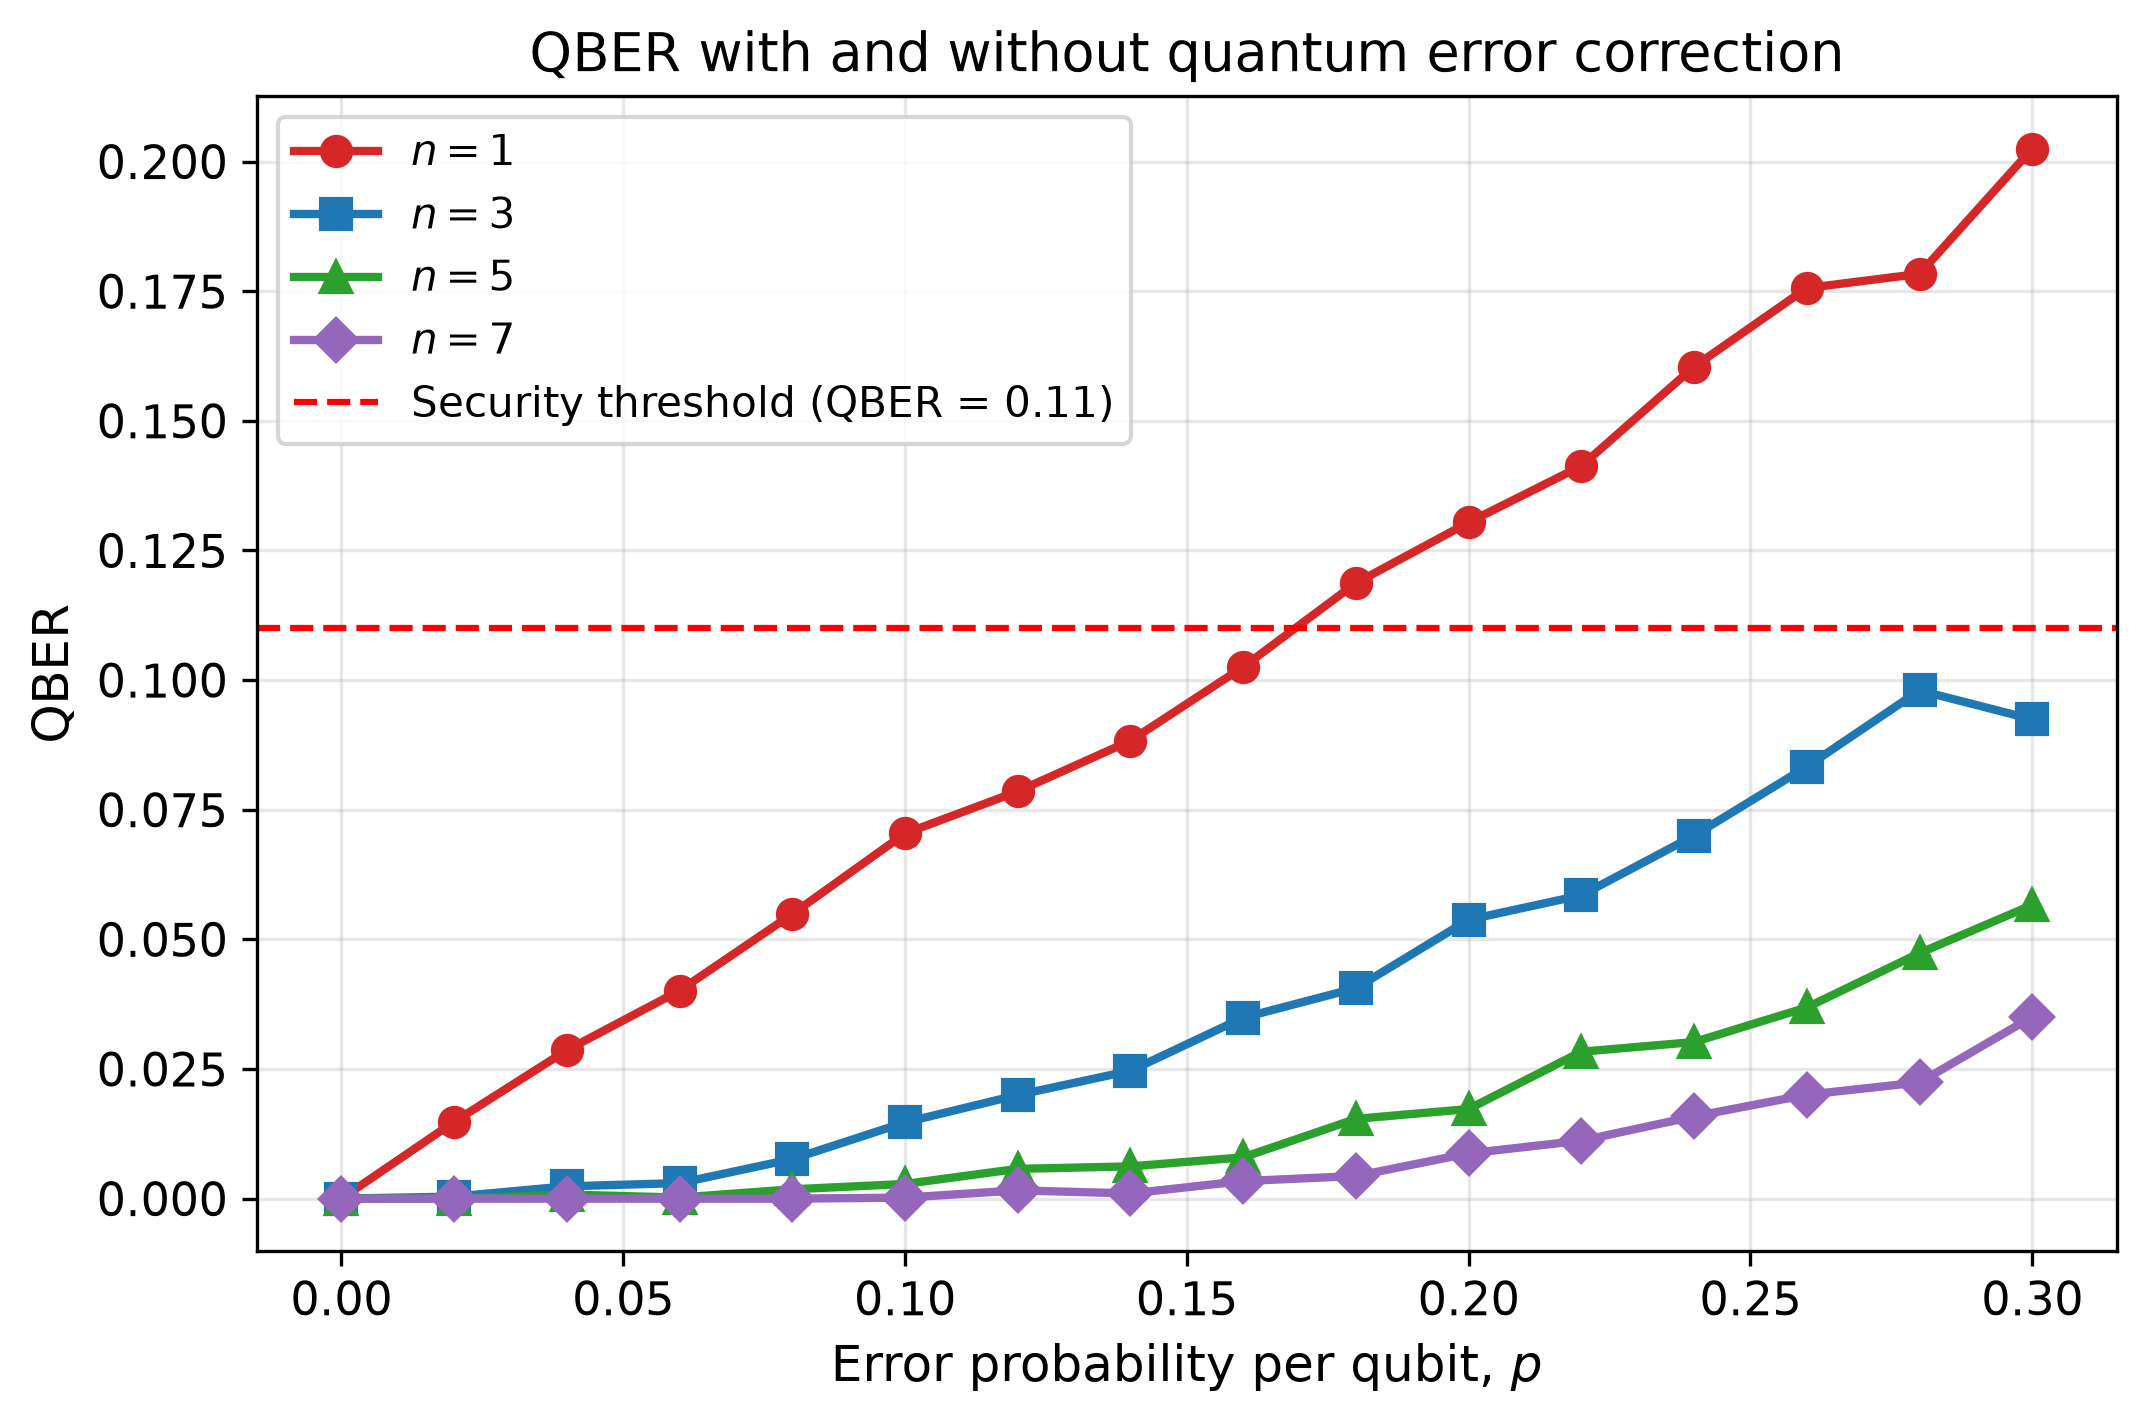
\includegraphics[width=\columnwidth]{../figs/qber_vs_p.png}
\caption{QBER en función de $p$ para $n=1,3,5,7$. La línea punteada marca el
umbral de seguridad ($\mathrm{QBER}=0.11$).}
\label{fig:qber}
\end{figure}

El comportamiento se explica por el mecanismo de votación descrito en la
Sección~\ref{sec:metodo}: al enviar el mismo valor varias veces y decidir por
mayoría, un error aislado no altera el resultado y se requiere que fallen más de
la mitad de las copias para perder el dato. Las pequeñas oscilaciones observadas
al final del barrido con $n=3$ son compatibles con la variabilidad estadística del
muestreo.

\subsection{Compromiso entre corrección y \textit{overhead}}

La Fig.~\ref{fig:tasa} muestra la contraparte del resultado anterior. Si la
corrección redujera el QBER sin costo, bastaría con aplicar el código más grande
disponible; la figura demuestra lo contrario. La curva sin corrección cae
abruptamente y se anula desde $p=0.18$, mientras que las curvas de $n=3$, $5$ y
$7$ arrancan en $0.333$, $0.200$ y $0.143$, respectivamente, y descienden con
suavidad. Las curvas se cruzan entre sí, lo que confirma que ningún tamaño de
código es superior en todos los regímenes.

\begin{figure}[!t]
\centering
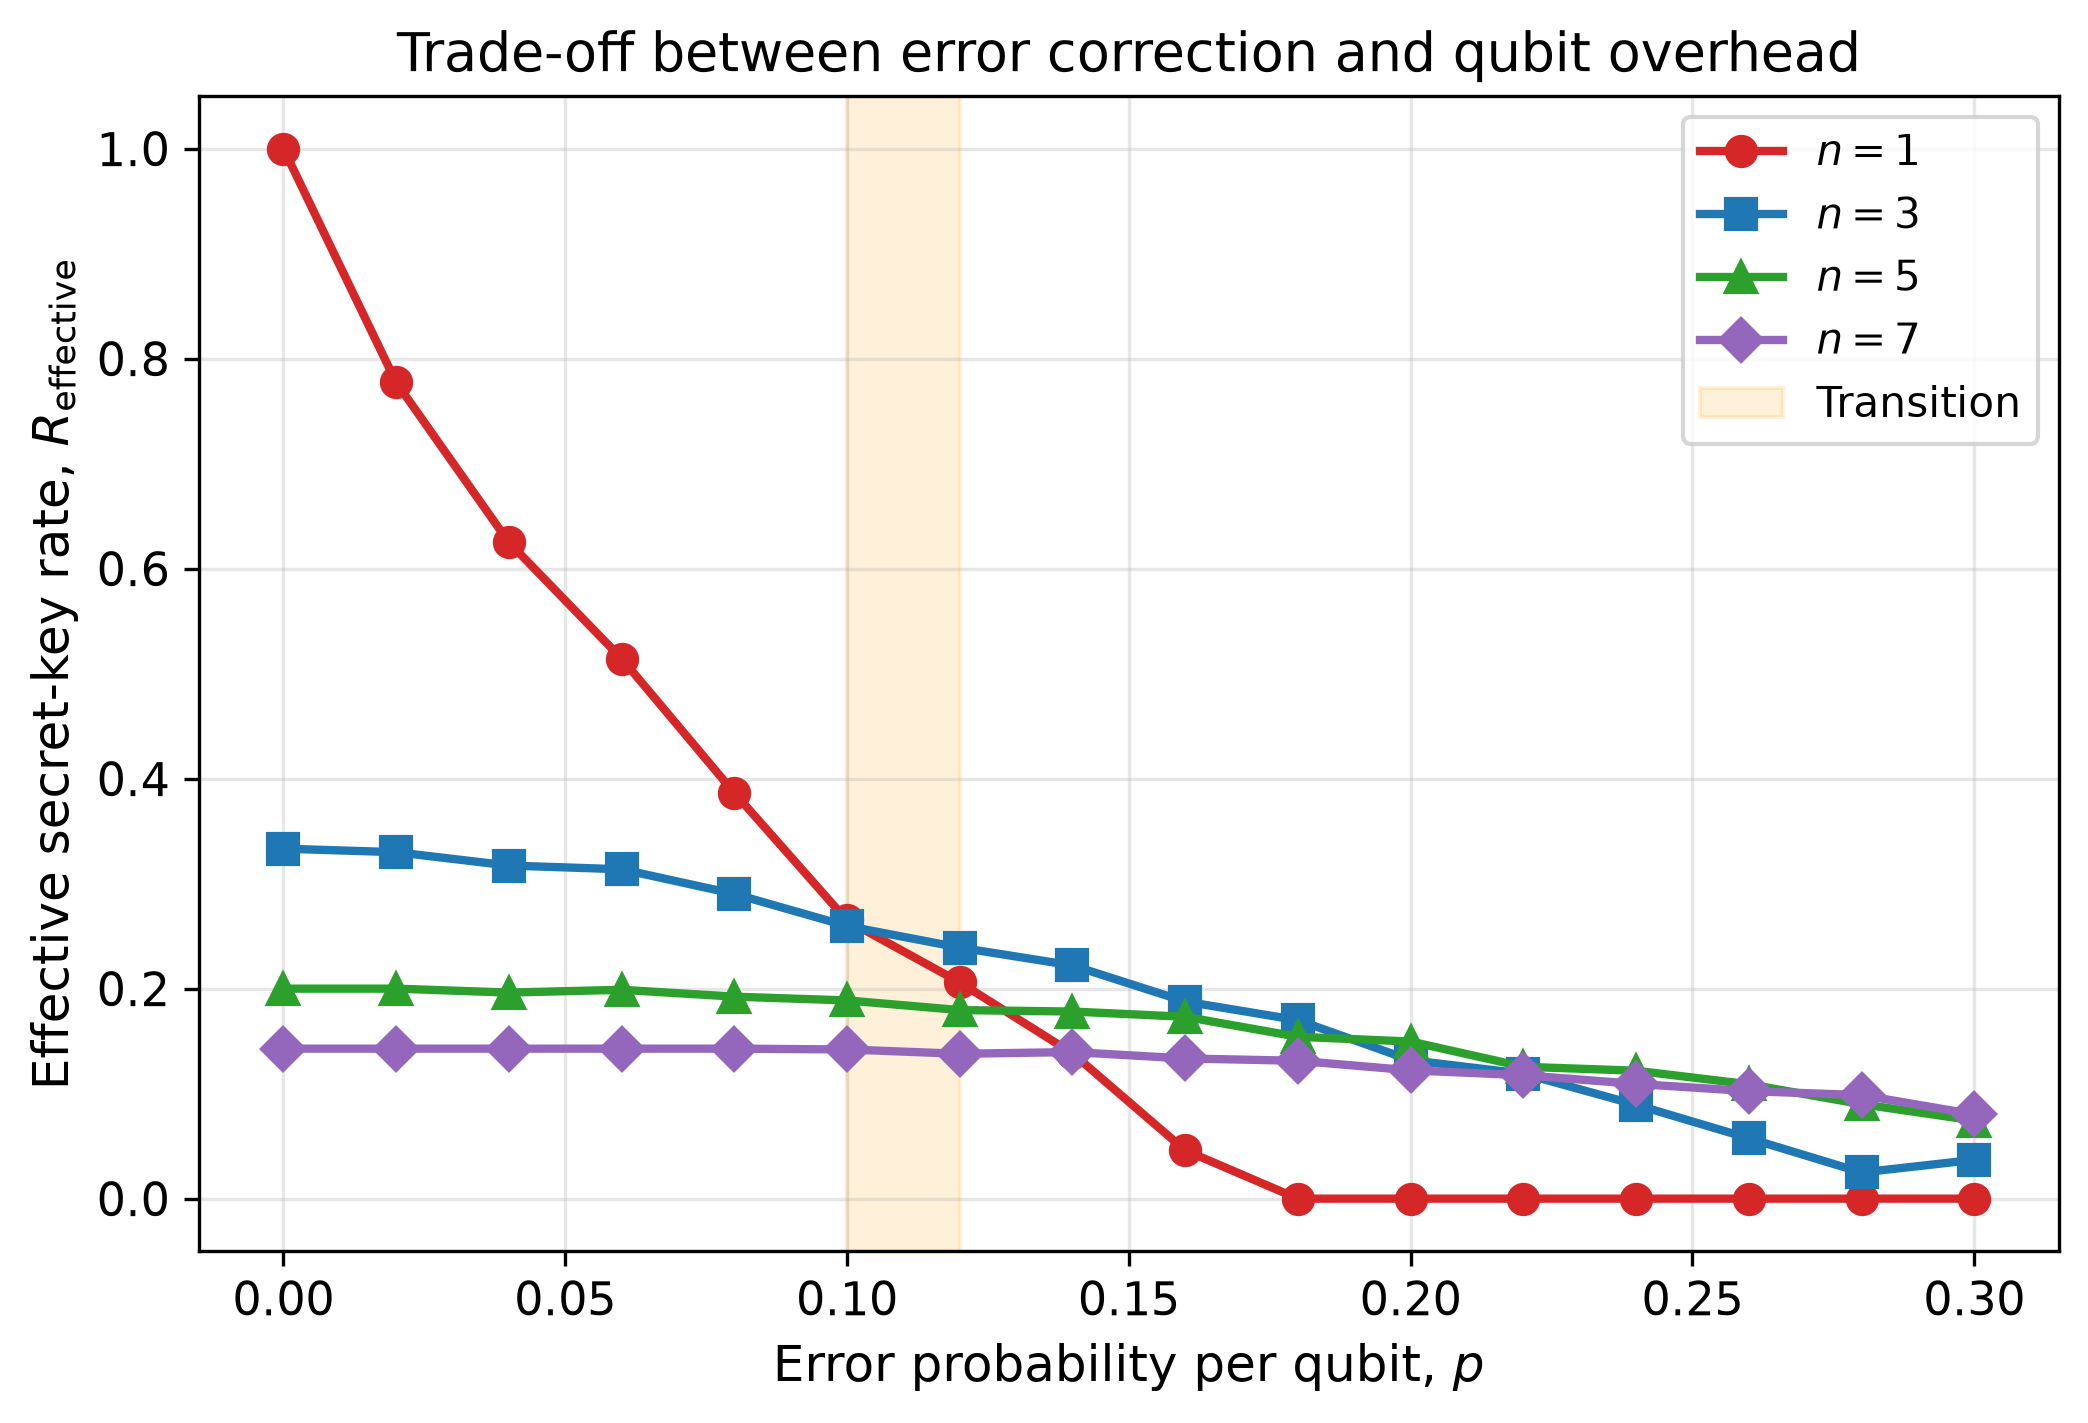
\includegraphics[width=\columnwidth]{../figs/tasa_efectiva_vs_p.png}
\caption{Tasa de clave efectiva $R_{\text{efectiva}}$ en función de $p$ para
$n=1,3,5,7$, calculada con \eqref{eq:efectiva}. La banda sombreada señala la
región de transición entre la operación sin corrección y el código $n=3$.}
\label{fig:tasa}
\end{figure}

La Tabla~\ref{tab:optimo} resume la decisión óptima para cada régimen de ruido.
Hasta $p=0.10$ conviene no aplicar corrección; entre $0.12$ y $0.18$ el óptimo es
$n=3$; entre $0.20$ y $0.26$, $n=5$; y desde $0.28$, $n=7$. El costo de
equivocarse es apreciable: en $p=0.12$, emplear $n=7$ exigiría más del doble de
qubits físicos por qubit lógico y entregaría una tasa de $0.138$ frente a
$0.239$; en $p=0.18$, operar sin corrección entrega una tasa nula.

\begin{table}[!t]
\renewcommand{\arraystretch}{1.15}
\caption{Tamaño de código óptimo por rango de ruido}
\label{tab:optimo}
\centering
\begin{tabular}{@{}cccc@{}}
\toprule
$p$ & $n^{*}$ & $R_{\text{efectiva}}(p,n^{*})$ & Régimen \\
\midrule
$0.00$--$0.10$ & 1 & $1.000$--$0.265$ & Sin QEC \\
$0.12$--$0.18$ & 3 & $0.239$--$0.170$ & Repetición \\
$0.20$--$0.26$ & 5 & $0.150$--$0.109$ & Repetición \\
$0.28$--$0.30$ & 7 & $0.099$--$0.080$ & Repetición \\
\bottomrule
\end{tabular}
\end{table}

\subsection{Mapa de calor $(p,n)$}

La Fig.~\ref{fig:mapa} presenta la misma información como mapa de calor. La
transición de colores sintetiza el hallazgo: en la fila $n=1$ se observa un
degradado rápido desde el amarillo ($p=0$) hasta el morado uniforme desde
$p=0.16$, donde la tasa se anula, mientras que las filas restantes permanecen en
tonos azules y morados a lo largo de todo el eje, lo que indica que su rendimiento
varía poco con el ruido. La celda más clara de cada columna se desplaza
escalonadamente: $n=1$ hasta $p=0.10$, $n=3$ desde $0.12$, $n=5$ desde $0.20$ y
$n=7$ desde $0.28$. Esa diagonal descendente responde la pregunta de
investigación: el tamaño de código óptimo aumenta con el ruido.

\begin{figure*}[!t]
\centering
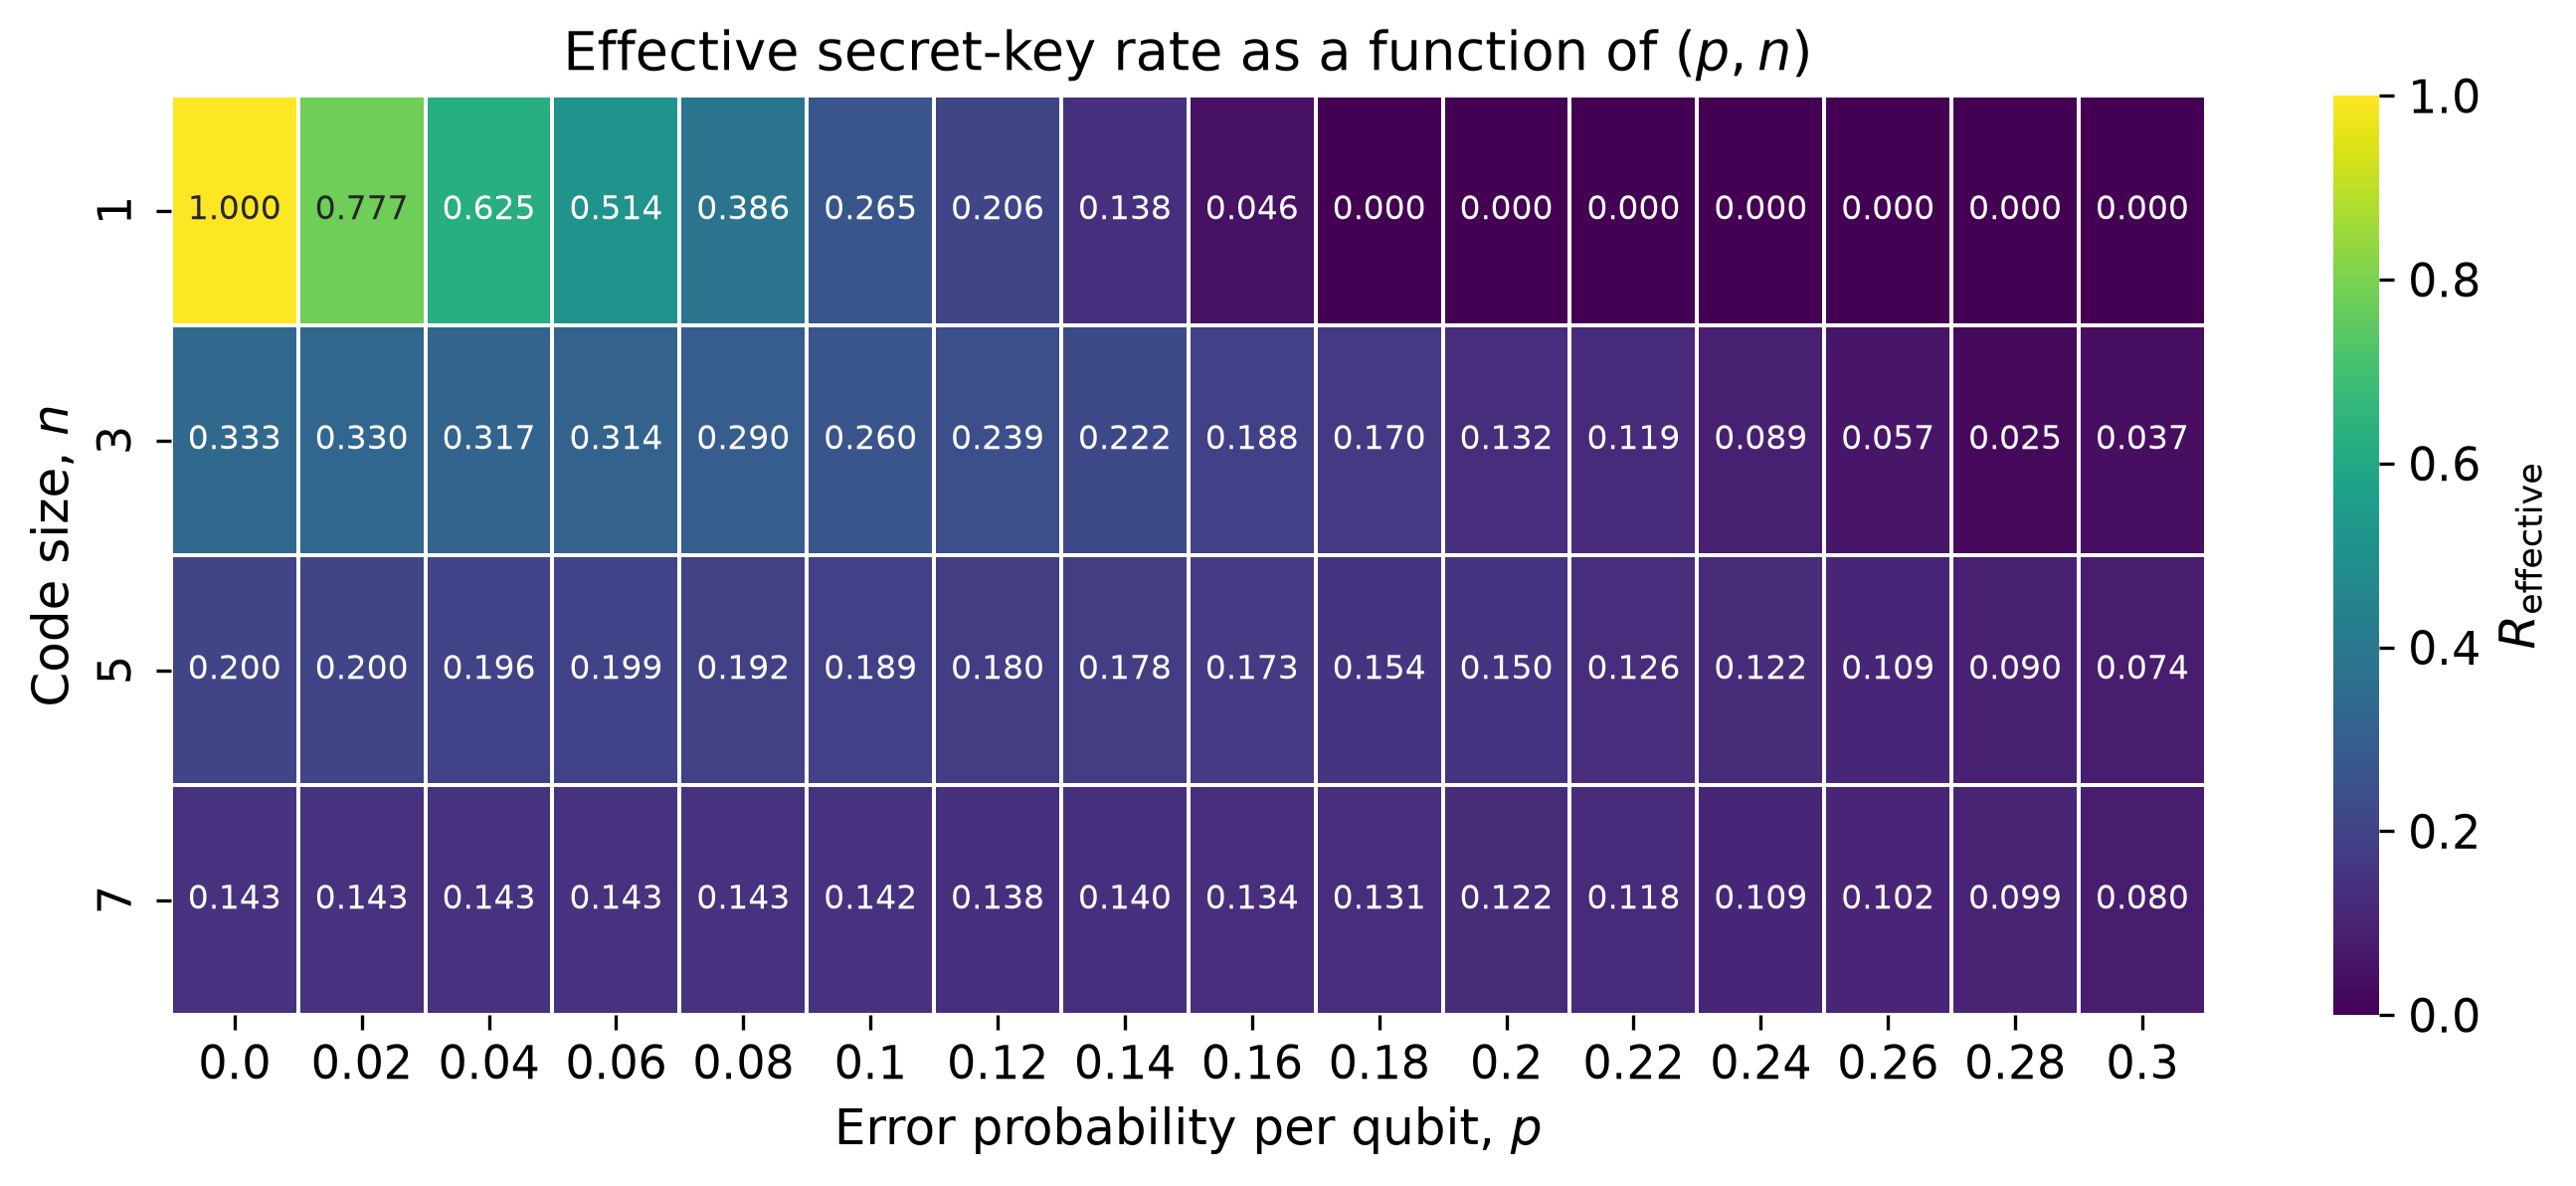
\includegraphics[width=\textwidth]{../figs/mapa_calor.png}
\caption{Tasa de clave efectiva en función de $(p,n)$; el color más claro indica
mayor tasa. La celda más brillante de cada columna señala el código óptimo para
ese nivel de ruido.}
\label{fig:mapa}
\end{figure*}

\subsection{Experimento de control: redundancia vs. corrección}
\label{sec:control}

Los resultados anteriores muestran que el QBER disminuye con el código de
repetición, pero no separan la contribución de la redundancia de la de la
corrección activa. Para aislar ambos efectos se compararon dos escenarios con
\(n=3\), \(p=0.15\), \(N=2000\) y la misma semilla (2026): A) cadena completa con
medición del síndrome y corrección; B) solo codificación, canal y decodificación
por mayoría. Ambos compartieron el mismo bit lógico, el mismo estado ruidoso y
las mismas extracciones aleatorias del decodificador. La Tabla~\ref{tab:control}
resume el resultado; los scripts están disponibles en
\texttt{control\_experiment/} del repositorio.

\begin{table}[!t]
\renewcommand{\arraystretch}{1.15}
\caption{Experimento de control con \(n=3\), \(p=0.15\) y \(N=2000\). Ambos
escenarios comparten semilla, estados ruidosos y extracciones del decodificador.}
\label{tab:control}
\centering
\begin{tabular}{@{}lccc@{}}
\toprule
Escenario & QBER & Error est. & Errores/\(N\) \\
\midrule
Con QEC & 0.0315 & 0.0039 & 63/2000 \\
Sin QEC & 0.0315 & 0.0039 & 63/2000 \\
Diferencia & 0.0000 & 0.0000 & 0 \\
\bottomrule
\end{tabular}
\end{table}

Los dos escenarios son idénticos: mismo QBER, mismos 63 errores y cero pares
discordantes. El síndrome fue trivial en 2000 de 2000 iteraciones y no se aplicó
ninguna corrección. La igualdad se explica porque, en la base \(Z\), corregir un
bit volteado y votar por mayoría producen la misma decisión. Para este código y
este canal,
\begin{equation}
\mathrm{QBER}_{A}=\mathrm{QBER}_{B}=3q^{2}(1-q)+q^{3},
\label{eq:control}
\end{equation}
donde \(q=2p/3\). Con \(p=0.15\), \(q=0.10\), \eqref{eq:control} predice
\(0.028\), compatible con el \(0.0315\) observado. La reducción proviene, por
tanto, de la redundancia estructurada y no de la corrección por síndrome.

\subsection{Implicaciones para la ciberseguridad}

Los resultados tienen dos consecuencias prácticas. La primera es la extensión
del rango operativo: sin corrección, el enlace deja de generar clave en
$p\approx0.165$; con $n=3$, el umbral no se alcanza ni siquiera en $p=0.30$. Dado
que la probabilidad de error crece en primera aproximación con la distancia
recorrida en la fibra, ese margen se traduce en un alcance útil cercano al doble.
La segunda es el ahorro de hardware: aplicar sistemáticamente el código más
protector derrocha recursos, mientras que elegir $n^{*}(p)$ permite obtener más
clave con menos qubits. Desde la perspectiva de la integridad del análisis, este
criterio evita además prometer una capacidad de generación que el enlace no puede
sostener.

Estos resultados dialogan con los antecedentes revisados. La integración de
cifrado y corrección propuesta por \cite{jha2024} reduce el costo fijo de etapas
separadas, mientras que la frontera $n^{*}(p)$ reduce el costo variable asociado
al tamaño del bloque; ambos enfoques son complementarios. La demostración de
corrección bajo umbral en 105 qubits \cite{acharya2025} valida la QEC en
hardware, aunque en un régimen distinto: allí se persigue la fidelidad de un
computador tolerante a fallos, con decenas o centenas de qubits físicos por qubit
lógico, mientras que en un enlace de QKD basta proteger el bit transmitido. Por
su parte, las métricas de fidelidad de \cite{zheng2024} y la validación en BB84 de
\cite{jayachandran2025} resultan consistentes con la tendencia aquí observada,
aunque ninguno de esos trabajos construye la frontera de optimalidad.

Conviene precisar el alcance de estas conclusiones. Los valores reportados
corresponden a un canal depolarizante estacionario, a fuentes de fotón único y a
detectores ideales, y la cota de \eqref{eq:shor} describe el régimen asintótico.
En un enlace real, la atenuación y el desalineamiento producen tasas de error
mayores, y el análisis de clave finita introduce penalizaciones adicionales que
reducen la tasa efectiva. Asimismo, el código de repetición protege frente a
errores de bit y no frente a errores de fase, de modo que los resultados no son
extrapolables sin más a códigos que corrigen ambos tipos de error. La frontera
$n^{*}(p)$ debe entenderse, por tanto, como una guía de dimensionamiento dentro
del modelo estudiado y no como un valor de operación para un enlace específico.

El experimento de control precisa el alcance de la contribución. Para el código
de repetición de tres qubits, la corrección por síndrome y la votación por
mayoría son matemáticamente equivalentes; la mejora del QBER proviene de la
redundancia estructurada y no de una superioridad «mágica» de la QEC. El valor de
este trabajo está, por tanto, en cuantificar el compromiso entre protección y
\textit{overhead} —la frontera \(n^{*}(p)\)— y no en postular un mecanismo de
corrección distinto. Una ventaja propia de la QEC requeriría códigos que corrijan
errores \(X\) y \(Z\), como el de Steane \cite{steane1996}, y una medición
proyectiva del síndrome; ambos aspectos quedan como trabajo futuro.

% ============================================================
% CONCLUSIÓN
% ============================================================
\section{Conclusión}
\label{sec:conclusion}

El presente trabajo cuantificó el compromiso entre corrección de errores
cuánticos y tasa de clave segura en el protocolo BB84 sobre un canal
depolarizante. La simulación con QuTiP de códigos de repetición permitió
establecer que no existe un tamaño de código universalmente óptimo: para
$p \leq 0.10$ conviene operar sin corrección, entre $0.12$ y $0.18$ el óptimo es
$n=3$, entre $0.20$ y $0.26$ lo es $n=5$, y desde $0.28$ domina $n=7$.

La reducción del QBER se atribuye, sin embargo, a la redundancia estructural del
código. El experimento de control con \(n=3\), \(p=0.15\) y 2000 bits, con semilla
y estados compartidos, produjo \(0.0315\) con y sin corrección y cero correcciones
activadas; para el código de repetición, el síndrome y la votación por mayoría son
operacionalmente equivalentes. La redundancia no solo reduce el QBER en más de un
orden de magnitud en el régimen moderado, sino que desplaza el umbral de
seguridad más allá de $p=0.30$, lo que aproximadamente duplica la tolerancia al
ruido del enlace. Al mismo tiempo, el \textit{overhead} impone un costo que hace
desaconsejable sobredimensionar el código: la elección de $n$ debe derivarse del
ruido esperado y no de la disponibilidad de recursos. La contribución es la
frontera \(n^{*}(p)\), no la atribución de la mejora al síndrome.

Las conclusiones están acotadas al modelo implementado: canal depolarizante,
fuentes y detectores ideales, régimen asintótico y códigos de repetición de hasta
siete qubits. Como trabajo futuro se propone incorporar pérdidas y desfase en el
canal, evaluar códigos estabilizadores que corrijan errores \(X\) y \(Z\) (por
ejemplo, el de Steane) con medición proyectiva del síndrome, y analizar la fuga
de información a través de los síndromes, aspectos que podrían reducir la tasa
efectiva aquí reportada.

% ============================================================
% REFERENCIAS (IEEE)
% ============================================================
\begin{thebibliography}{99}

\bibitem{shor1997} P. W. Shor, ``Polynomial-time algorithms for prime
factorization and discrete logarithms on a quantum computer,'' \emph{SIAM J.
Comput.}, vol. 26, no. 5, pp. 1484--1509, Oct. 1997, doi:
10.1137/S0097539795293172.

\bibitem{mosca2018} M. Mosca, ``Cybersecurity in an era with quantum computers:
Will we be ready?,'' \emph{IEEE Security \& Privacy}, vol. 16, no. 5, pp.
38--41, Sep.--Oct. 2018, doi: 10.1109/MSP.2018.3761723.

\bibitem{regenscheid2026} A. Regenscheid, \emph{Transition to Post-Quantum
Cryptography Standards}, NIST IR 8547. Gaithersburg, MD, USA: National Institute
of Standards and Technology, 2026, doi: 10.6028/NIST.IR.8547.

\bibitem{nist2024a} National Institute of Standards and Technology,
\emph{Module-Lattice-Based Key-Encapsulation Mechanism Standard}, FIPS 203.
Gaithersburg, MD, USA: U.S. Dept. of Commerce, 2024, doi:
10.6028/NIST.FIPS.203.

\bibitem{nist2024b} National Institute of Standards and Technology,
\emph{Module-Lattice-Based Digital Signature Standard}, FIPS 204. Gaithersburg,
MD, USA: U.S. Dept. of Commerce, 2024, doi: 10.6028/NIST.FIPS.204.

\bibitem{bennett1984} C. H. Bennett and G. Brassard, ``Quantum cryptography:
Public key distribution and coin tossing,'' in \emph{Proc. IEEE Int. Conf.
Comput., Syst. Signal Process.}, Bangalore, India, 1984, pp. 175--179.
Reimpresión: \emph{Theoretical Computer Science}, vol. 560, pp. 7--11, 2014, doi:
10.1016/j.tcs.2014.05.025.

\bibitem{gisin2002} N. Gisin, G. Ribordy, W. Tittel, and H. Zbinden, ``Quantum
cryptography,'' \emph{Rev. Mod. Phys.}, vol. 74, no. 1, pp. 145--195, Jan. 2002,
doi: 10.1103/RevModPhys.74.145.

\bibitem{shor2000} P. W. Shor and J. Preskill, ``Simple proof of security of the
BB84 quantum key distribution protocol,'' \emph{Phys. Rev. Lett.}, vol. 85, no.
2, pp. 441--444, Jul. 2000, doi: 10.1103/PhysRevLett.85.441.

\bibitem{steane1996} A. M. Steane, ``Error correcting codes in quantum theory,''
\emph{Phys. Rev. Lett.}, vol. 77, no. 5, pp. 793--797, Jul. 1996, doi:
10.1103/PhysRevLett.77.793.

\bibitem{scarani2009} V. Scarani, H. Bechmann-Pasquinucci, N. J. Cerf, M.
Du\v{s}ek, N. L\"utkenhaus, and M. Peev, ``The security of practical quantum key
distribution,'' \emph{Rev. Mod. Phys.}, vol. 81, no. 3, pp. 1301--1350, Sep.
2009, doi: 10.1103/RevModPhys.81.1301.

\bibitem{xu2020} F. Xu, X. Ma, Q. Zhang, H.-K. Lo, and J.-W. Pan, ``Secure
quantum key distribution with realistic devices,'' \emph{Rev. Mod. Phys.}, vol.
92, no. 2, art. 025002, Jun. 2020, doi: 10.1103/RevModPhys.92.025002.

\bibitem{nielsen2010} M. A. Nielsen and I. L. Chuang, \emph{Quantum Computation
and Quantum Information}, 10th anniversary ed. Cambridge, U.K.: Cambridge
University Press, 2010, doi: 10.1017/CBO9780511976667.

\bibitem{terhal2015} B. M. Terhal, ``Quantum error correction for quantum
memories,'' \emph{Rev. Mod. Phys.}, vol. 87, no. 2, pp. 307--346, Apr. 2015,
doi: 10.1103/RevModPhys.87.307.

\bibitem{acharya2025} R. Acharya \emph{et al.} [Google Quantum AI and
Collaborators], ``Quantum error correction below the surface code threshold,''
\emph{Nature}, vol. 638, no. 8052, pp. 920--926, Feb. 2025, doi:
10.1038/s41586-024-08449-y.

\bibitem{fowler2012} A. G. Fowler, M. Mariantoni, J. M. Martinis, and A. N.
Cleland, ``Surface codes: Towards practical large-scale quantum computation,''
\emph{Phys. Rev. A}, vol. 86, no. 3, art. 032324, Sep. 2012, doi:
10.1103/PhysRevA.86.032324.

\bibitem{jha2024} N. Jha, A. Parakh, and M. Subramaniam, ``Joint encryption and
error correction for secure quantum communication,'' \emph{Sci. Rep.}, vol. 14,
art. 24542, 2024, doi: 10.1038/s41598-024-75212-8.

\bibitem{zheng2024} G. Zheng, W. He, G. Lee, and L. Jiang, ``Near-optimal
performance of quantum error correction codes,'' \emph{Phys. Rev. Lett.}, vol.
132, no. 25, art. 250602, Jun. 2024, doi: 10.1103/PhysRevLett.132.250602.

\bibitem{jayachandran2025} R. Jayachandran and D. Malathi, ``Experimental
validation of quantum error correction in BB84 for secure quantum
communication,'' \emph{Int. J. Theor. Phys.}, vol. 64, no. 11, art. 310, 2025,
doi: 10.1007/s10773-025-06148-6.

\bibitem{johansson2012} J. R. Johansson, P. D. Nation, and F. Nori, ``QuTiP: An
open-source Python framework for the dynamics of open quantum systems,''
\emph{Comput. Phys. Commun.}, vol. 183, no. 8, pp. 1760--1772, Aug. 2012, doi:
10.1016/j.cpc.2012.02.021.

\end{thebibliography}

\end{document}
